\documentclass[a4paper,12pt]{article}

\usepackage{graphicx}
\graphicspath{{figures/}}
\usepackage{geometry}
\geometry{textwidth=426pt}
\usepackage{tabularx, ragged2e}
\usepackage{mathtools}
\usepackage{multicol}
\usepackage{titlesec}

\titleformat{\section}{\fontsize{11}{15}\bfseries}{\Roman{section}}{1em}{}
\titleformat{\paragraph}{\normalfont}{\textbf{\theparagraph.}}{0.5em}{}
\titlespacing*{\paragraph}{1.5em}{1.em}{1.em}
\counterwithout{paragraph}{section}
\setcounter{secnumdepth}{4}


\begin{document}

%\scshape
\centering
\onecolumn

\noindent
\begin{minipage}[]{0.7\textwidth}
\large{Practicum 1 $-$ group A \\Enzymatic activity of nitrophenyl-phosphatase}\par \vspace{0.1em}
\footnotesize{Quantitative cell analysis \& tissue engineering}\vspace{0.6em}
\flushleft
\begin{tabularx}{\widthof{\large{MAKING TITLES IN \LaTeX}}}{X l}
Team:  & Céline Duchaine\\
& Leen van Kerckhoven \\
& Lucas Comyn \\
& Vincent Belpaire \\
%Role: & Student at USI\\
%Supervisor: & Julien Prokofiev\\
Date: & October 5, 2022
\end{tabularx}


\end{minipage}% PUT THIS HERE!
\begin{minipage}[]{0.3\textwidth}
\flushright{

\includegraphics[width=3cm, keepaspectratio]{logo_ghent.png} \par \vspace{0.1cm}
\texttt{Faculty of engineering and architecture}
}
\end{minipage}

\flushleft

\section{Standard curve for nitrophenol}

\paragraph{Make a plot of the absorbance versus concentration and calculate the trendline. ($E=bx+a$ with $x=$ nitrophenol concetration) And calculate the concentration of P01.}

\begin{figure}[!ht]
    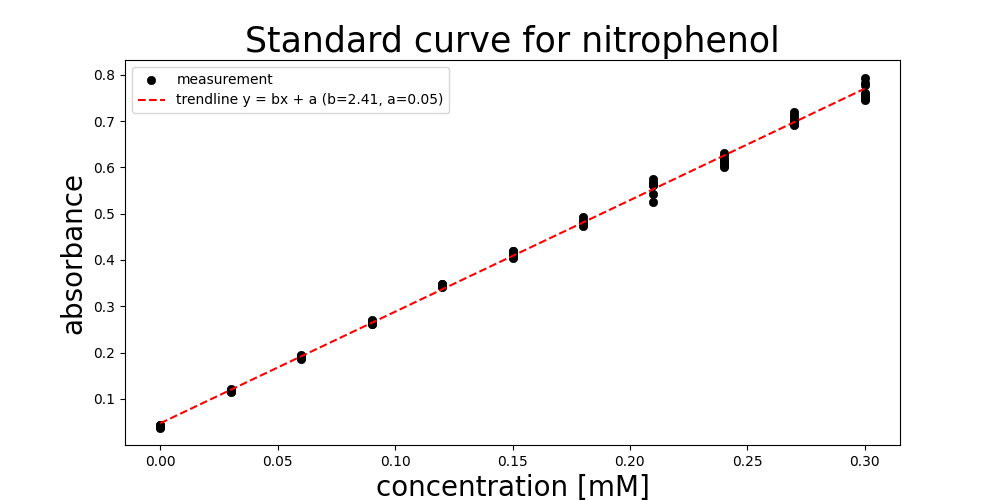
\includegraphics[scale=0.5]{fig1.png}
    \centering
\end{figure}

The estimated concentration of PO1 is 0.01743 mM. (We made the mean of all of the results to estimate it's concentration.)

\section{Enzymatic activity as a function of substrate concentration}

\paragraph{Plot the enzymatic activity (as absorbance after 30 minutes (Y-axis)) 
against the substrate concentration (X-axis) and display $R^2$.}

\begin{figure}[!ht]
    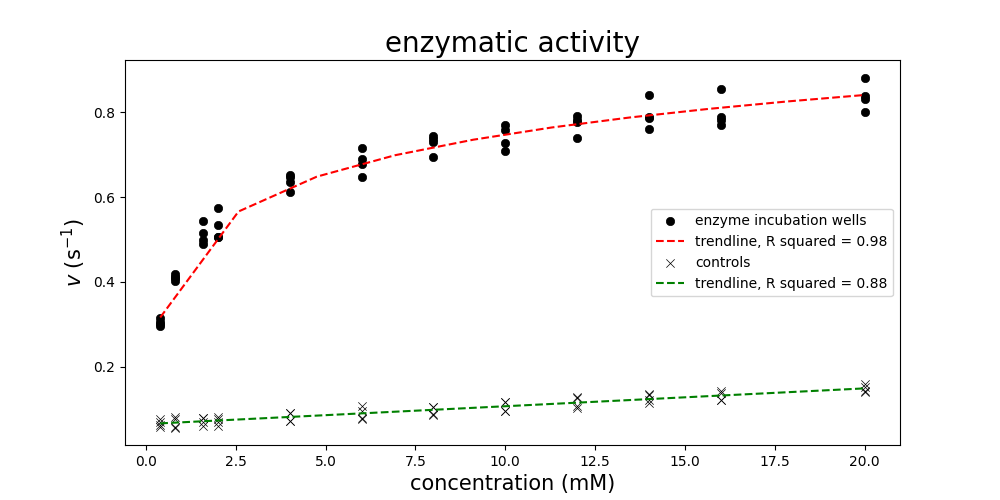
\includegraphics[scale=0.5]{fig2_1.png}
    \centering
\end{figure}

\paragraph{Lineweaver-Burk plot: $\frac{1}{v}$ (Y-axis) against $\frac{1}{[S]}$ (X-axis) and display $R^2$. 
Formula of Michaëlis Menten:\[v=V_{\text{max}}\frac{[S]}{K_m+[S]}\] \[\frac{1}{v}=\frac{1}{V_{\text{max}}}\left(\frac{K_m}{[S]}+1\right)\]}

\begin{figure}[!ht]
    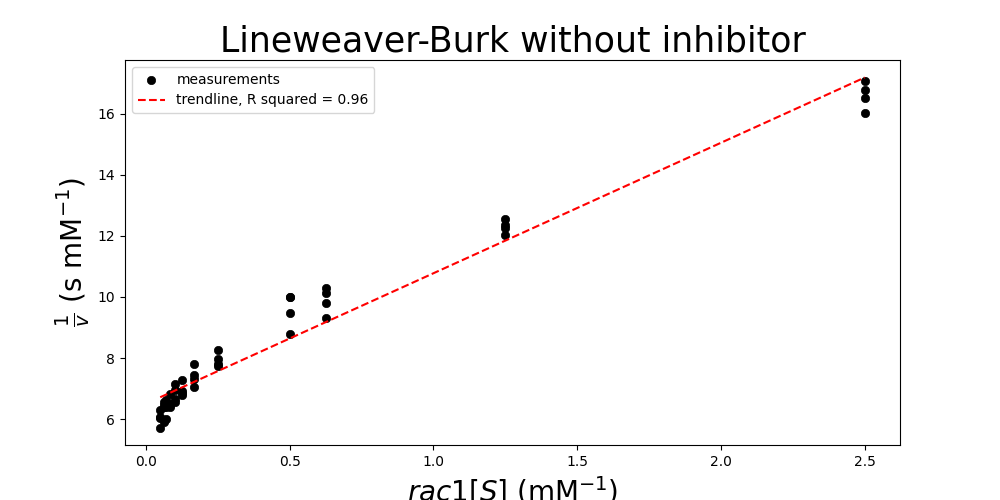
\includegraphics[scale=0.5]{fig2_2.png}
    \centering
\end{figure}

\paragraph{Eadie-Hofstee plot: $\frac{v}{[S]}$ (X-axis) against $v$ (Y-axis) and display $R^2$. \[v=-K_m\frac{v}{[S]}+V_{\text{max}}\]}

\begin{figure}[!ht]
    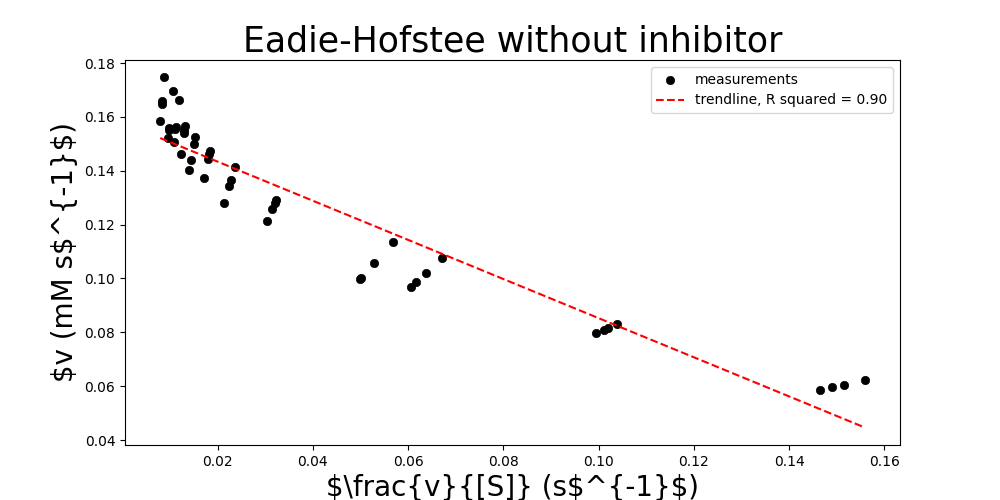
\includegraphics[scale=0.5]{fig2_3.png}
    \centering
\end{figure}

\paragraph{Hanes-Woolf plot: $\frac{[S]}{v}$ (Y-axis) against $[S]$ (X-axis) and display $R^2$. \[\frac{[S]}{v}=\frac{[S]}{V_{\text{max}}}+\frac{K_m}{V_{\text{max}}}\]}

\begin{figure}[!ht]
    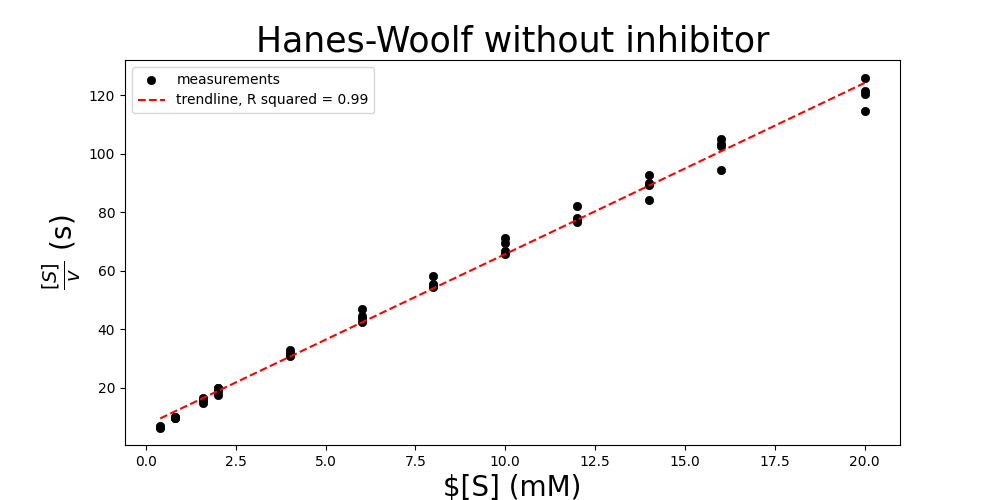
\includegraphics[scale=0.5]{fig2_4.png}
    \centering
\end{figure}

\paragraph{Calculate $K_m$-value (molarity of substrate in incubation mixture) and $V_{\text{max}}$ (formed nitrophenol (mg) per 30 minutes) for every plot. Do you observe 
differences? Why? 
}

q2.2 Lineweaver-Burk plot: Vmax = 0.15 mM/s, Km = 0.66 mM
q2.3 Eadie-Hofstee plot: Vmax = 0.16 mM/s, Km = 0.73 mM
q2.4 Hanes-Woolf plot: Vmax = 0.17 mM/s, Km = 1.22 mM

\section{Enzymatic activity in the presence of an inhibitor}

\paragraph{Plot the enzymatic activity (as absorbance after 30 minutes (Y-axis)) 
against the substrate concentration (X-axis). Add a trendline and $R^2$}

\begin{figure}[!ht]
    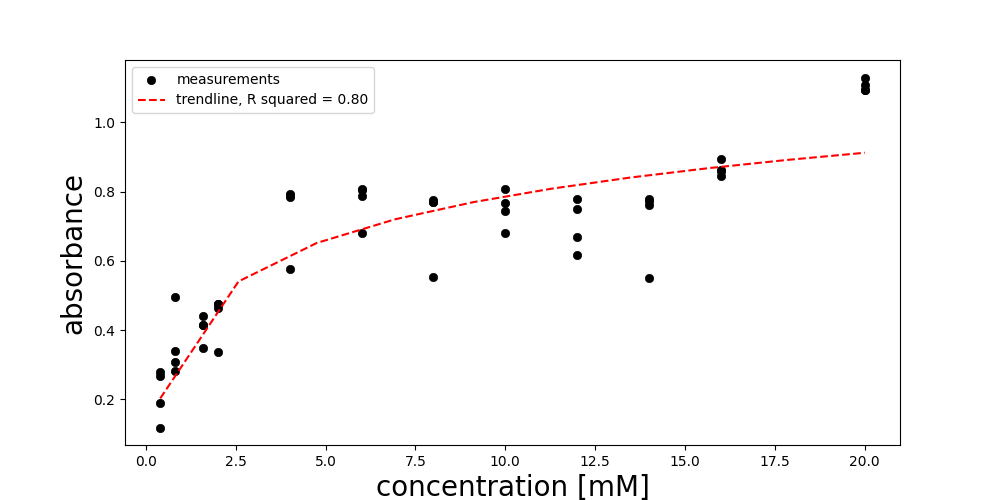
\includegraphics[scale=0.5]{fig3_1.png}
    \centering
\end{figure}

\paragraph{Lineweaver-Burk plot: $\frac{1}{v}$ (Y-axis) against $\frac{1}{[S]}$ (X-axis).}

\begin{figure}[!ht]
    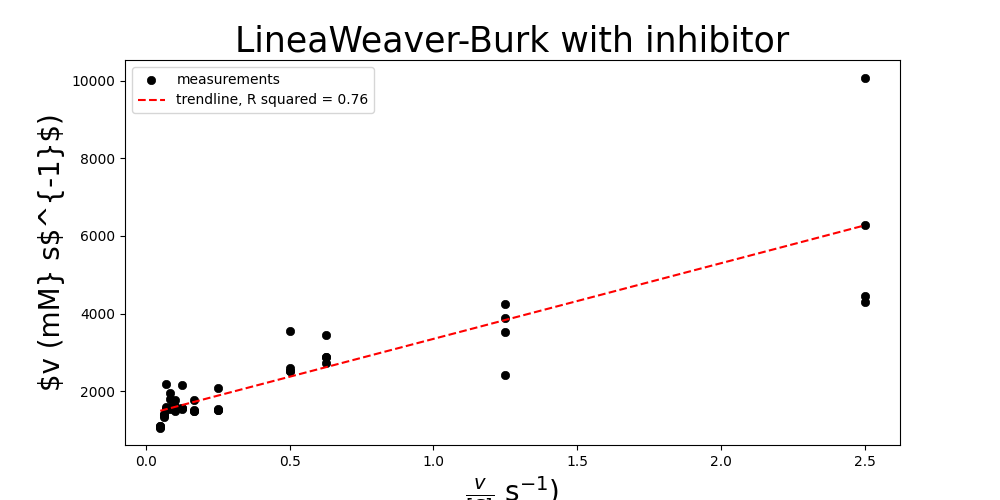
\includegraphics[scale=0.5]{fig3_2.png}
    \centering
\end{figure}

\paragraph{Eadie-Hofstee plot: $\frac{v}{[S]}$ (X-axis) against $v$ (Y-axis).}

\begin{figure}[!ht]
    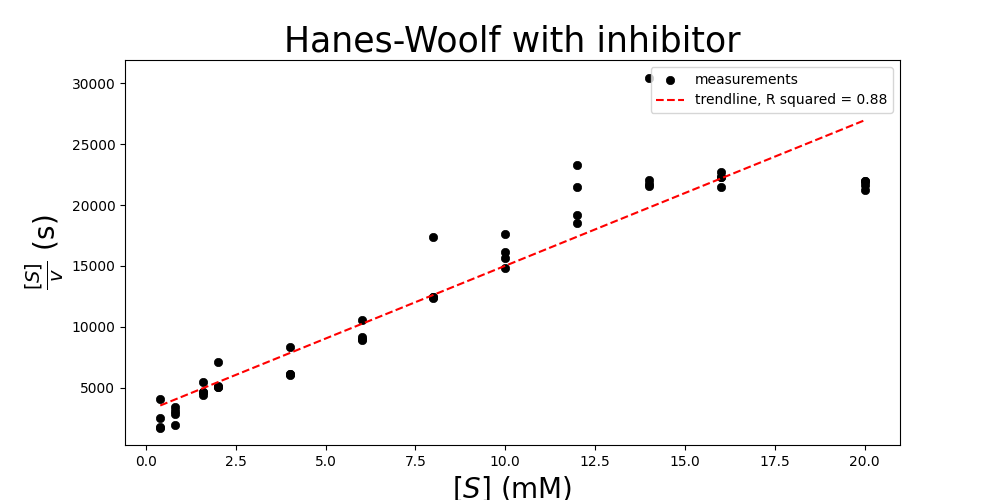
\includegraphics[scale=0.5]{fig3_4.png}
    \centering
\end{figure}

\paragraph{Hanes-Woolf plot: $\frac{[S]}{v}$ (Y-axis) against $[S]$ (X-axis).}

\begin{figure}[!ht]
    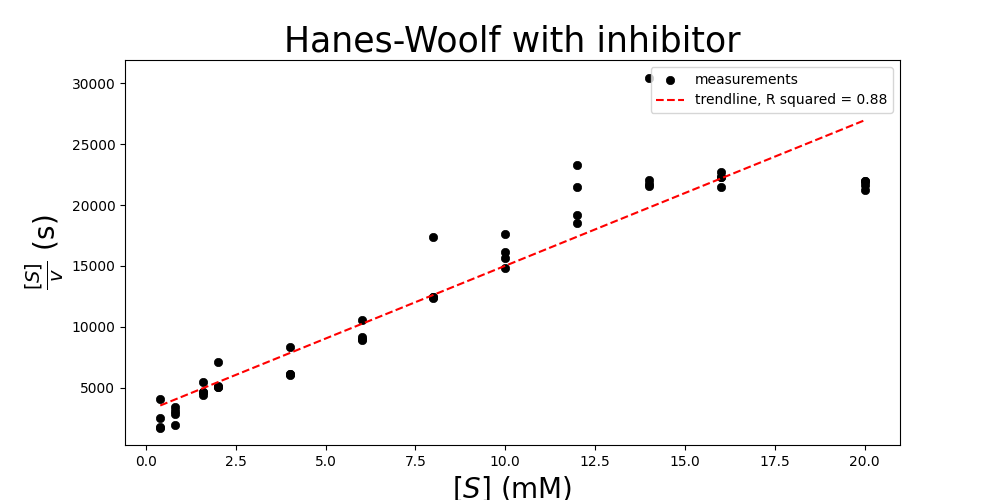
\includegraphics[scale=0.5]{fig3_4.png}
    \centering
\end{figure}

\paragraph{Calculate $K_m$-value (molarity of substrate in incubation mixture) and $V_{\text{max}}$ (formed nitrophenol (mg) per 30 minutes) for every plot.}
Km represents the amount of substrate required to bind half of the avaible enzyme.
Vmax is the theoretical maximum rate for the reaction.

q3.2 Lineweaver-Burk plot: Vmax = 0.000716 mM/s, Km = 1.40 mM
q3.3 Eadie-Hofstee plot: Vmax = 0.000701 mM/s, Km = 1.08 mM
q3.4 Hanes-Woolf plot: Vmax = 0.000836 mM/s, Km = 2.55 mM

\paragraph{Is the inhibitor competitive or non-competitive? Motivate your answer.}

Answer\\

\end{document}
